\begin{center}
    Questions
\end{center}
\begin{enumerate}
    \item What are property rights?
    \item Which of the following represents the true economic cost of production when firms produce goods that cause negative externalities?
    \item Private Costs:
    \item Which of the following is an example of a positive externality?
    \item Suppose the current market equilibrium output of $Q_1$ is not the economically efficient output because of an externality.
    The economically efficient output is $Q_2$.
    In that case, the diagram shows:
    \begin{figure}[h!]
        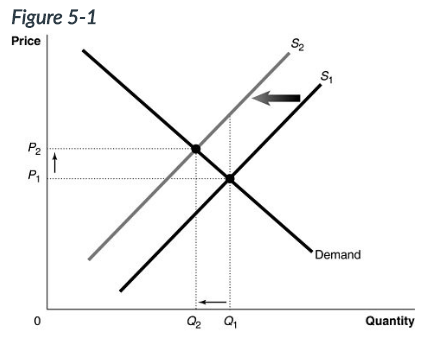
\includegraphics{images/Question5.png}
        \caption{Figure 5-1 shows a market with an externality. The current market equilibrium output of $Q_1$ is not the economically efficient output. The economically efficient output is $Q_2$.}
    \end{figure}
    \item Refer to figure 5-1.
    If because of an externality, the economically efficient output is $Q_2$ and not the current equilibrium output of $Q_1$, what does $S_2$ represent?
    \item The deadweight loss due to the externality is represented by the area:
    \begin{figure}[h!]
        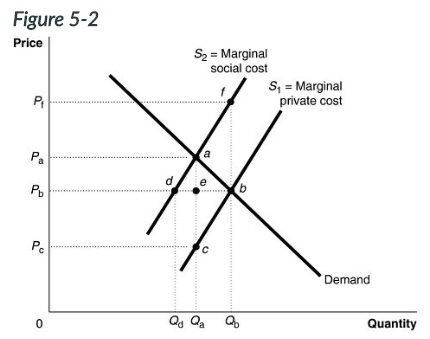
\includegraphics{images/fig5-2.png}
        \caption{Figure 5-2 shows a market with a negative externality.}
    \end{figure}
    \item Pollution is an example of a:
    \item The cost borne by a producer in the production of a good or service is called:
    \item What does $D_1$ represent?
    \begin{figure}[h!]
        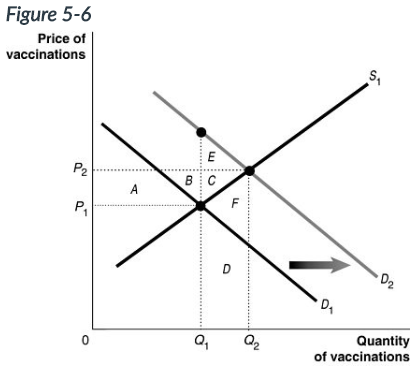
\includegraphics{images/fig5-6.png}
        \caption{Figure 5-6 shows the market for measles vaccinations, a product  whose use generates positive externalities.}
    \end{figure}
    \item Explain how mandatory seat belt laws may reduce the negative externalities of risky behavior.
    \item If there is pollution in producing a product, then the market equilibrium price:
    \item Consider the following characteristics:
    \begin{itemize}
        \item low transaction costs
        \item small levels of pollution
        \item high levels of pollution
        \item clear assignment of property rights
    \end{itemize}
    Which of the above are assumptions behind the Coase Theorem?
    \item What is the economic efficient level of pollution reduction?
    \begin{figure}[h!]
        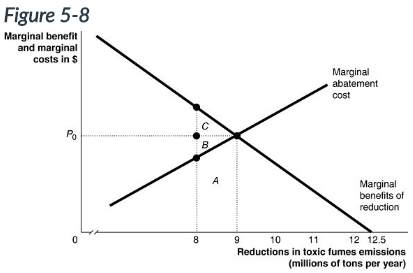
\includegraphics{images/fig5-8.png}
        \caption{Consider a chemical plant that discharges toxic fumes over a nearby community.
        To reduce the emissions of toxic fumes the firm can install pollution abatement devices.
        Figure 5-8 shows the marginal benefit and the marginal cost from reducing the toxic fumes emissions.}
    \end{figure}
    \item Refer to figure 5-8.
    Suppose the emissions reduction target is currently established at 8 million tons.
    What is the area that represents the cost of eliminating an additional 1 million tons?
    \item State and local governments subsidize college students with grants and low-interest loans.
    The loans and subsidies are example of:
    \item Refer to figure 5-13.
    The efficient equilibrium quantity of gasoline is \_\_\_ million gallons per month.
    \begin{figure}[h!]
        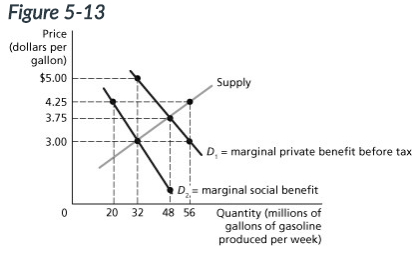
\includegraphics{images/fig5-13.png}
        \caption{Figure 5-13 illustrates the market for gasoline before and after the government imposes a tax to bring about the efficient level of gasoline production.}
    \end{figure}
    \item Refer to figure 5-13.
    The market equilibrium quantity of gasoline is \_\_\_ million gallons per month.
\end{enumerate}

\begin{center}
    Answers
\end{center}
\begin{enumerate}
    \item The rights individuals or firms have to the exclusive use of their property, including the right to but or sell it.
    \item The social cost of production.
    \item Are borne by producers of a good while social costs are borne by society at large.
    \item Planting trees along a sidewalk which add beauty and shade.
    \item The effect of a negative externality in the production of a good.
    \item The market supply curve reflecting marginal social cost.
    \item abf.
    \item Negative externality.
    \item Private cost.
    \item The demand curve reflecting private benefits.
    \item Seat belt laws help reduce injuries related to motor accidents.
    This results in less costs in medical bills and less time spent in hospital, or could save the lives of those involved.
    \item Is too low and equilibrium quantity is to high.
    \item A and D.
    \item 9 million tons.
    \item A
    \item Pigovian subsidies.
    \item 32
    \item 48
    \item \$5.00
    \item \$1.25
    \item A good that is rivalrous and excludable.
    \item Nonrivalry and nonexludability.
    \item True.
    \item $P_2 - P_0$
\end{enumerate}